\section{Introduction}\label{sec:introduction}

Bias is the overrepresentation of a particular topics in an individuals social media feed. This bias could be representative
of the individuals interests, or it could be representative of the interests of the social media platform. The latter is where
the notion of bias becomes complicated. Is my feed bias if it shows me only posts on topic A, if the only posts on the 
social media platform are of topic A? For the purpose of this report, we will take the stand that bias refers to the deviation from
the "norm".\\
\textbf{Bias Definition:} the deviation of a users social media feed from the distribution of available posts.

Bias in social media can easily be seen by comparing users' social media. In fact, I can show this with ease by just taking a look at my
Instagram's "Explore page", and compare it to another's.
\newpage
\begin{figure}[htbp]
    \centering
    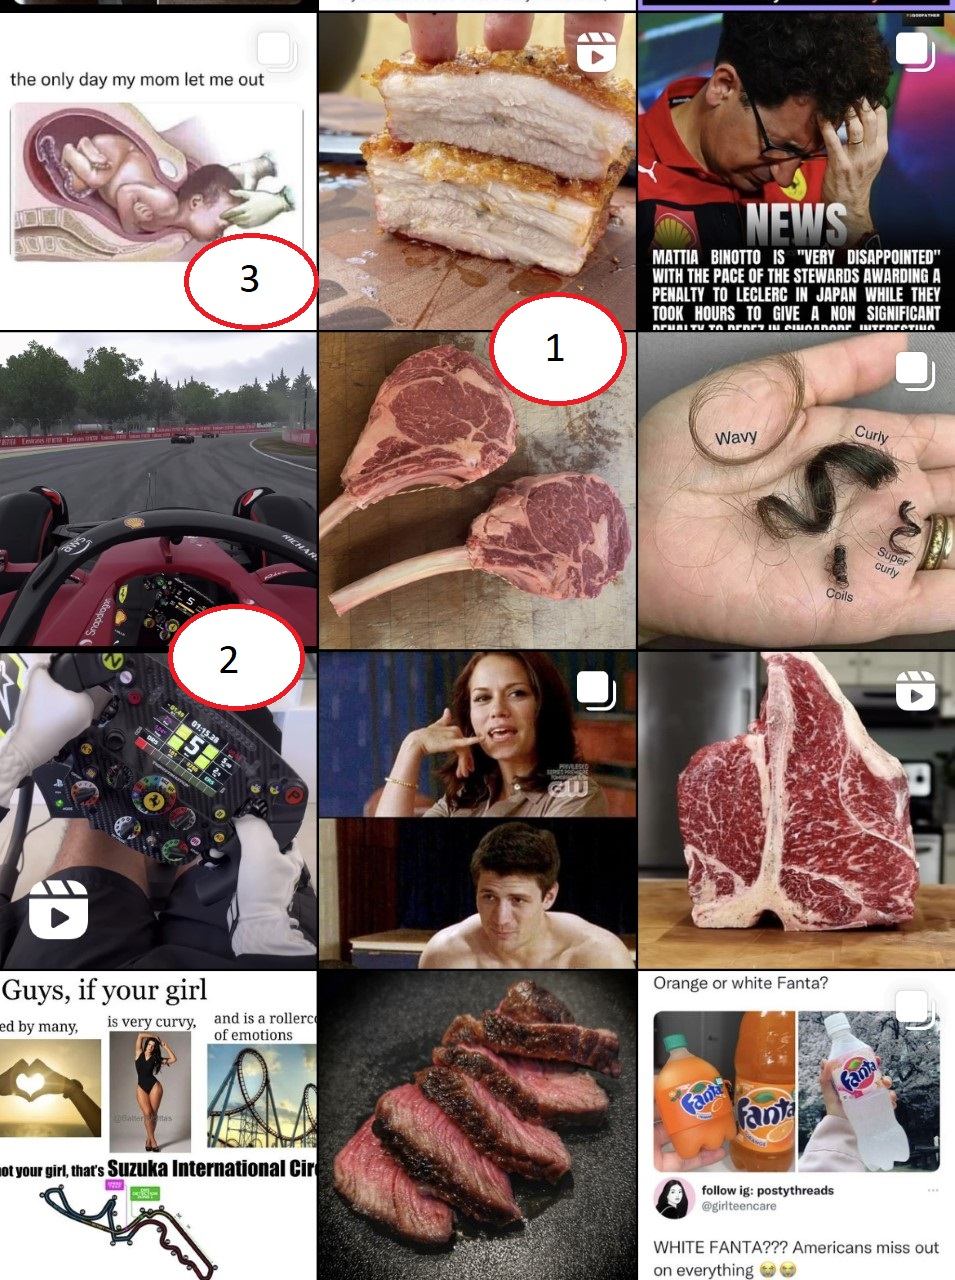
\includegraphics[height=80mm]{../images/ig4u.jpg}
    \caption{My Instagram for you page}
    \label{fig:ig4u}
\end{figure}

Here we can notice a few common themes/biases: 1. Food, 2. Formula 1, 3. Memes. We want to be able to identify these biases for users
so they can get an overview of the type of content they are receiving from social media.\\
With social media recommender systems programmed to entice users with content they will enjoy (\cite{recommenderSystems}), it is common for similar groups of posts
to be observed by a user if they have recently liked, commented, or viewed similar posts (\cite{instagram_how_nodate}).\\
Although the content in the feed only shows a small number of topics, we can not guarantee bias, as we are unaware of the 
distribution of all posts on the platform.

\newpage

\begin{figure}[htbp]
    \centering
    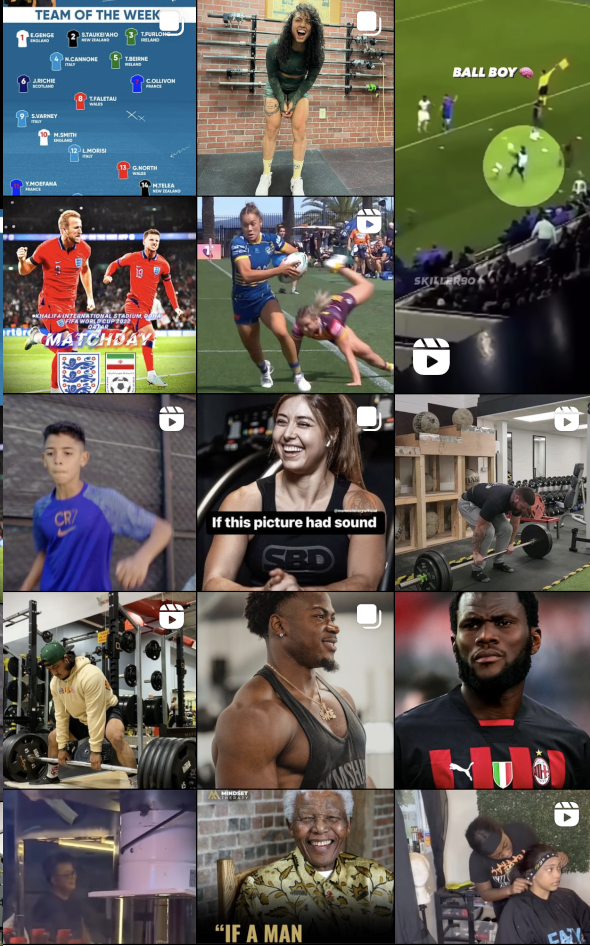
\includegraphics[height=80mm]{../images/ig4u2.png}
    \caption{Another Instagram for you page}
    \label{fig:ig4u2}
\end{figure}

This for you page shows very different content to the previous one; there is a lot of sport/gym posts and absolutely no
posts on food. This helps to show that bias exists in social media.\\
\textbf{Proof}:
Let us assume that no bias exists in these examples.
Then simultaneously, the following must be true:
\begin{itemize}
    \item The posts in figure \ref{fig:ig4u} is representative of the entire distribution of posts on the social media site.
    \item The posts in figure \ref{fig:ig4u2} is representative of the entire distribution of posts on the social media site.
\end{itemize}

This, trivially, can not be true due to the fact that the two pages show differing content. $\qed$\\\\

This project attempts to show how bias is affected by how a user interacts with social media.
There are a couple of challenges to this project. The first being, even though we have a definition of bias,
we need a way to measure it. This involves creating a model to detect what topic a post is about and figuring
out how to identify the distribution of topics on a social media site. The second challenge is to setup rules that
represent different strategies users can use to interact with social media. We can then implement these rules
and analyse the change in topics over time.


\subsection{Related work}

\subsubsection{Pythia - \cite{Pythia}}
Pythia is an automated system for short text classification. It makes use of Wikipedia structure and articles to identify
topics of posts.
Essentially, "Wikipedia contains articles organized in various taxonomies, called categories". Pythia then goes on to use
this information as their training data as well as handling sparseness in posts on social media.

\subsubsection{Topic tracking of student-generated posts - \cite{TopicTracking}}
This paper proposes a solution for determining valuable information/topics discussed in student forums on online courses.
It uses a model called "Time Information-Emotion Behaviour Model" or otherwise called "TI-EBTM" to detect key topics discussions
, keeping in mind the progress of time throughout the forum.\\
Although this paper specializes in academic online forums, the approaches made could be relevant and useful for this project.

\subsubsection{Topic classification of blogs - \cite{husby2012topic}}
This paper uses Distant Supervision - 'an extension of the paradigm used by (\cite{snow}) for exploiting WordNet to extract hypernym (is-a) relations between entitities'
- to get training data via Wikipedia articles. Then trains their own designed model on this data to be able to classify topics via a
multi-class recognition model (69\% accuracy) and via a binary classification model (90\% accuracy).

\subsubsection{BERT - \cite{bertmodelling}}
This paper analyses BERT (as well as modified BERT models such as RoBERTa) and how they can be used for text classification.
The data used in this paper is a set of scientific papers that are classified into 7 different categories.\\

The paper shows that using a Feedforward Neural Network (FNN) on top of BERT can achieve a 91.76\% accuracy on the dataset.
This is a very high accuracy, and shows that BERT can be used for text classification.\\

\subsection{Objectives}

This project will require a topic detection model to be built and to perform some data analysis.
An extension for this project will be to create a Chrome Extension.

Below are the objectives for this project (Objectives in green are completed):

\begin{itemize}
    \item Build a topic detection model
    \begin{itemize}
        % make item green
        \item \textcolor{green}{Research possible models}
        \item \textcolor{green}{Gather data for model training}
        \item \textcolor{green}{Iterate over making and training models}
        \item Decide chosen model
        \item Train model on larger dataset
        \item Assess models accuracy and performance
        \item Include other information in the model (e.g. image/media attached in posts)
    \end{itemize}
    \item Data analysis
    \begin{itemize}
        \item Determine the distribution of topics on social media - aka the "norm"
        \item Create a set of rules to represent different strategies users can use to interact with social media
        \item Implement these rules and analyse the change in topics over time
        \item Compare the results of the rules to the "norm"
        \t\item This may require the use of a mathematical model to determine differences over time-series data
    \end{itemize}
    \item EXTENSION: Chrome Extension
    \begin{itemize}
        \item Design UI for extension
        \item Implement UI design
        \item Gather data from social media sites from the extensions frontend
        \item Create an API that receives post information and returns a set of most represented topics
        \item Connect extension to API
    \end{itemize}
\end{itemize}